\section{Experiments}
\label{sec:experiments}

\begin{figure*}[t]
  \centering  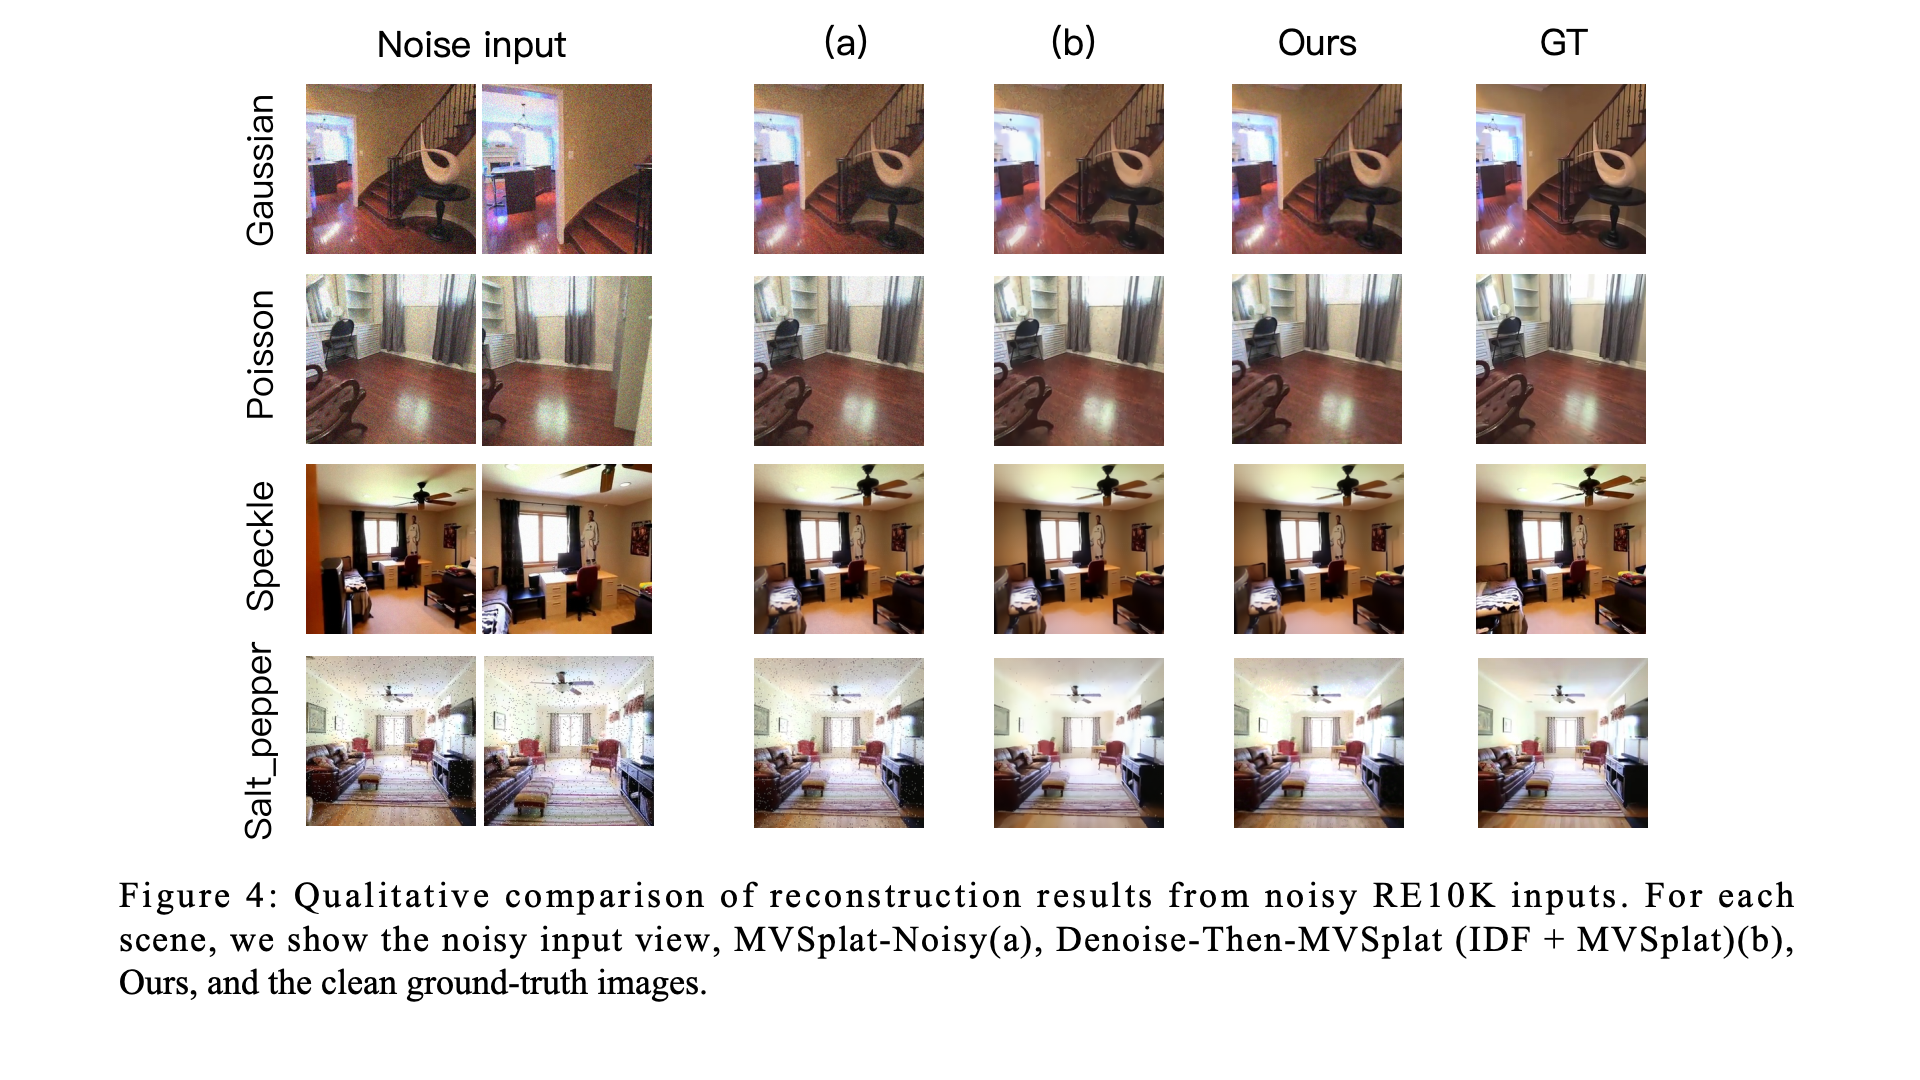
\includegraphics[width=1\linewidth, trim=0 50 0 20, clip]{figs/major_com_vis.png}
  
  \label{fig:major_com_vis}
\end{figure*}

In this section, we evaluate the proposed method on the noisy multi-view dataset constructed from RE10K. We first describe the experimental setup and baselines, then present overall results and qualitative analyses, and finally conduct ablation studies to examine the effect of key design choices.



\subsection{Experimental Settings}
\label{subsec:exp_settings}

\noindent \textbf{Datasets and protocol.}
We use RealEstate10K (RE10K). For each scene, we uniformly sample a fixed number of frames as multi-view inputs and synthesize noisy--clean pairs as in Sec.~\ref{subsec:noise_degradation_dataset}.
Specifically, we apply a single randomly sampled noise type (Gaussian, Poisson, speckle, or salt-and-pepper) with a randomly sampled intensity (within the specified ranges) to \emph{all} views of the scene in the 2D RGB domain, producing \(\tilde{I}^{\text{noise}}_{s,v}\) with clean targets \(I^{\text{GT}}_{s,v}\).
Splits are scene-level with no overlap across train/val/test.
Unless stated otherwise, we report results on both \emph{seen views} (training views) and \emph{novel views} extrapolated along the camera trajectory, to assess reconstruction and generalization jointly.

\noindent \textbf{Metrics.}
We report PSNR (\(\uparrow\)), SSIM (\(\uparrow\)), and LPIPS (\(\downarrow\)), averaged over the test set; we additionally break down performance on seen vs.\ novel views.

\noindent \textbf{Baselines.}
We compare: (i) \textbf{MVSplat-GT} (upper bound), trained and evaluated on clean RE10K; 
(ii) \textbf{MVSplat-Noisy}, the clean-trained MVSplat evaluated directly on noisy inputs without fine-tuning;
(iii) \textbf{Denoise-Then-MVSplat}, a two-stage pipeline applying IDF~\cite{kim2025idf} (official pretrained weights, default inference) per view and then feeding the restored images into clean-trained MVSplat~\cite{chen2024mvsplat}, without fine-tuning either module; and
(iv) \textbf{Ours (DenoiseSplat)}, an MVSplat-style feed-forward 3DGS model retrained on our noisy--clean benchmark with noisy inputs and clean 2D supervision, without test-time optimization.

\noindent \textbf{Efficiency.}
To assess potential overhead, we report runtime/memory under a unified setting (single GPU, 256$\times$256, 2 context views).
We discard the first 5 batches for warm-up and report the mean runtime; results are summarized in Tab.~\ref{tab:efficiency}.

\input{tabs/efficiency}




\begin{table}
  \centering
  \caption{%
    Overall reconstruction performance on the noisy RE10K test set. 
    We report average PSNR$\uparrow$, SSIM$\uparrow$, and LPIPS$\downarrow$ over all test views.
  }
  \label{tab:overall_results}
  \begin{tabular}{lccc}
    \toprule
    Method & PSNR $\uparrow$ & SSIM $\uparrow$ & LPIPS $\downarrow$ \\
    \midrule
    MVSplat-GT(upper bound)    & 26.38 & 0.869 & 0.128 \\
    MVSplat-Noisy              & 24.46 & 0.702 & 0.349 \\
    Denoise-Then-MVSplat (IDF) & 24.77 & 0.788 & 0.272 \\
    \textbf{Ours}              & \textbf{25.05} & \textbf{0.814} & \textbf{0.260} \\
    \bottomrule
  \end{tabular}
\end{table}



\begin{table*}[t]
  \centering
  \caption{%
    Ablation on the standard deviation $\sigma$ of Gaussian noise for our DenoiseSplat. 
    We report average performance on the noisy RE10K test set.
  }
  \label{tab:gaussian_ablation}
\begin{tabular}{l|ccc|ccc|ccc}
    \multirow{2}{*}{Methods} & \multicolumn{3}{|c|}{MVSplat-Noisy} & \multicolumn{3}{c|}{Denoise-Then-MVSplat} & \multicolumn{3}{c}{\textbf{DenoiseSplat(Ours)}}\\
    \cline{2-10}
     & PSNR & SSIM & LPIPS  &
       PSNR & SSIM & LPIPS  &
       PSNR $\uparrow$ & SSIM $\uparrow$ & LPIPS $\downarrow$ \\
    \noalign{\hrule height 1.0pt}
    $\sigma$ = 0.05 & 25.19 & 0.777 & 0.298 & 25.28 & 0.801 & 0.256 & 25.44 & 0.814 & 0.243\\
    $\sigma$ = 0.08 & 24.62 & 0.700 & 0.365 & 24.82 & 0.732 & 0.300 & 24.86 & 0.784 & 0.282\\
    $\sigma$ = 0.12 & 23.54 & 0.612 & 0.432 & 24.26 & 0.665 & 0.396 & 24.33 & 0.742 & 0.328\\
    $\sigma$ = 0.15 & 22.79 & 0.557 & 0.472 & 23.14 & 0.603 & 0.436 & 23.87 & 0.712 & 0.360\\
\end{tabular}

\end{table*}

\subsection{Main Results}
\label{subsec:main_results}



\noindent \textbf{Overall performance.}
Tab.~\ref{tab:overall_results} summarizes the reconstruction accuracy and perceptual quality on the noisy RE10K test set.
Among methods that operate on noisy inputs, \textbf{DenoiseSplat} achieves the strongest overall trade-off across PSNR, SSIM, and LPIPS, and reduces the gap to the clean-input upper bound \textbf{MVSplat-GT}.
In contrast, directly feeding noisy images to \textbf{MVSplat-Noisy} leads to a pronounced drop, most notably in SSIM and LPIPS, which is consistent with texture blurring and local structural inconsistencies under noise.
Introducing a strong 2D denoiser in \textbf{Denoise-Then-MVSplat} improves all three metrics compared to \textbf{MVSplat-Noisy}.
Nevertheless, a noticeable margin to \textbf{MVSplat-GT} remains, especially in perceptual quality, suggesting that view-independent 2D restoration does not fully preserve the cues needed for multi-view reconstruction under challenging noise.

\noindent \textbf{Seen vs. novel views.}
Novel-view synthesis is generally more sensitive to geometric uncertainty than seen-view reconstruction.
Consistent with this, \textbf{MVSplat-Noisy} exhibits a larger performance drop on novel views, indicating difficulty in maintaining reliable multi-view consistency when the inputs are corrupted.
\textbf{Denoise-Then-MVSplat} narrows this gap to some extent, but its novel-view quality can still be limited when the 2D denoiser introduces view-dependent artifacts or removes fine details that are important for matching.
By comparison, \textbf{DenoiseSplat} maintains more stable performance across seen and novel views, with a smaller gap between them, which is indicative of improved cross-view coherence when noise is handled within the 3D reconstruction pipeline.

\noindent \textbf{Qualitative comparisons.}
Fig.~4 visualizes representative examples from the noisy RE10K test set.
On scenes with rich textures and complex boundaries, \textbf{MVSplat-Noisy} often leaves visible residual noise and exhibits color shifts or localized distortions.
\textbf{Denoise-Then-MVSplat} typically yields cleaner appearances, but frequently softens edges and suppresses high-frequency details, especially at higher noise levels.
We further highlight recurring \emph{failure patterns} of this two-stage pipeline in Fig.~5, including over-smoothing of fine textures, halo/ringing near strong boundaries, and erosion of thin structures (e.g., wires or railings).
These effects are consistent with view-independent 2D restoration, which may remove or alter high-frequency cues in a manner that is not fully consistent across views, thereby weakening multi-view correspondence and boundary fidelity.
In comparison, \textbf{DenoiseSplat} removes most visible noise while better preserving boundary sharpness and texture details, producing more coherent renderings with fewer artifacts in novel view synthesis.

\begin{figure}[ht]
  \centering
  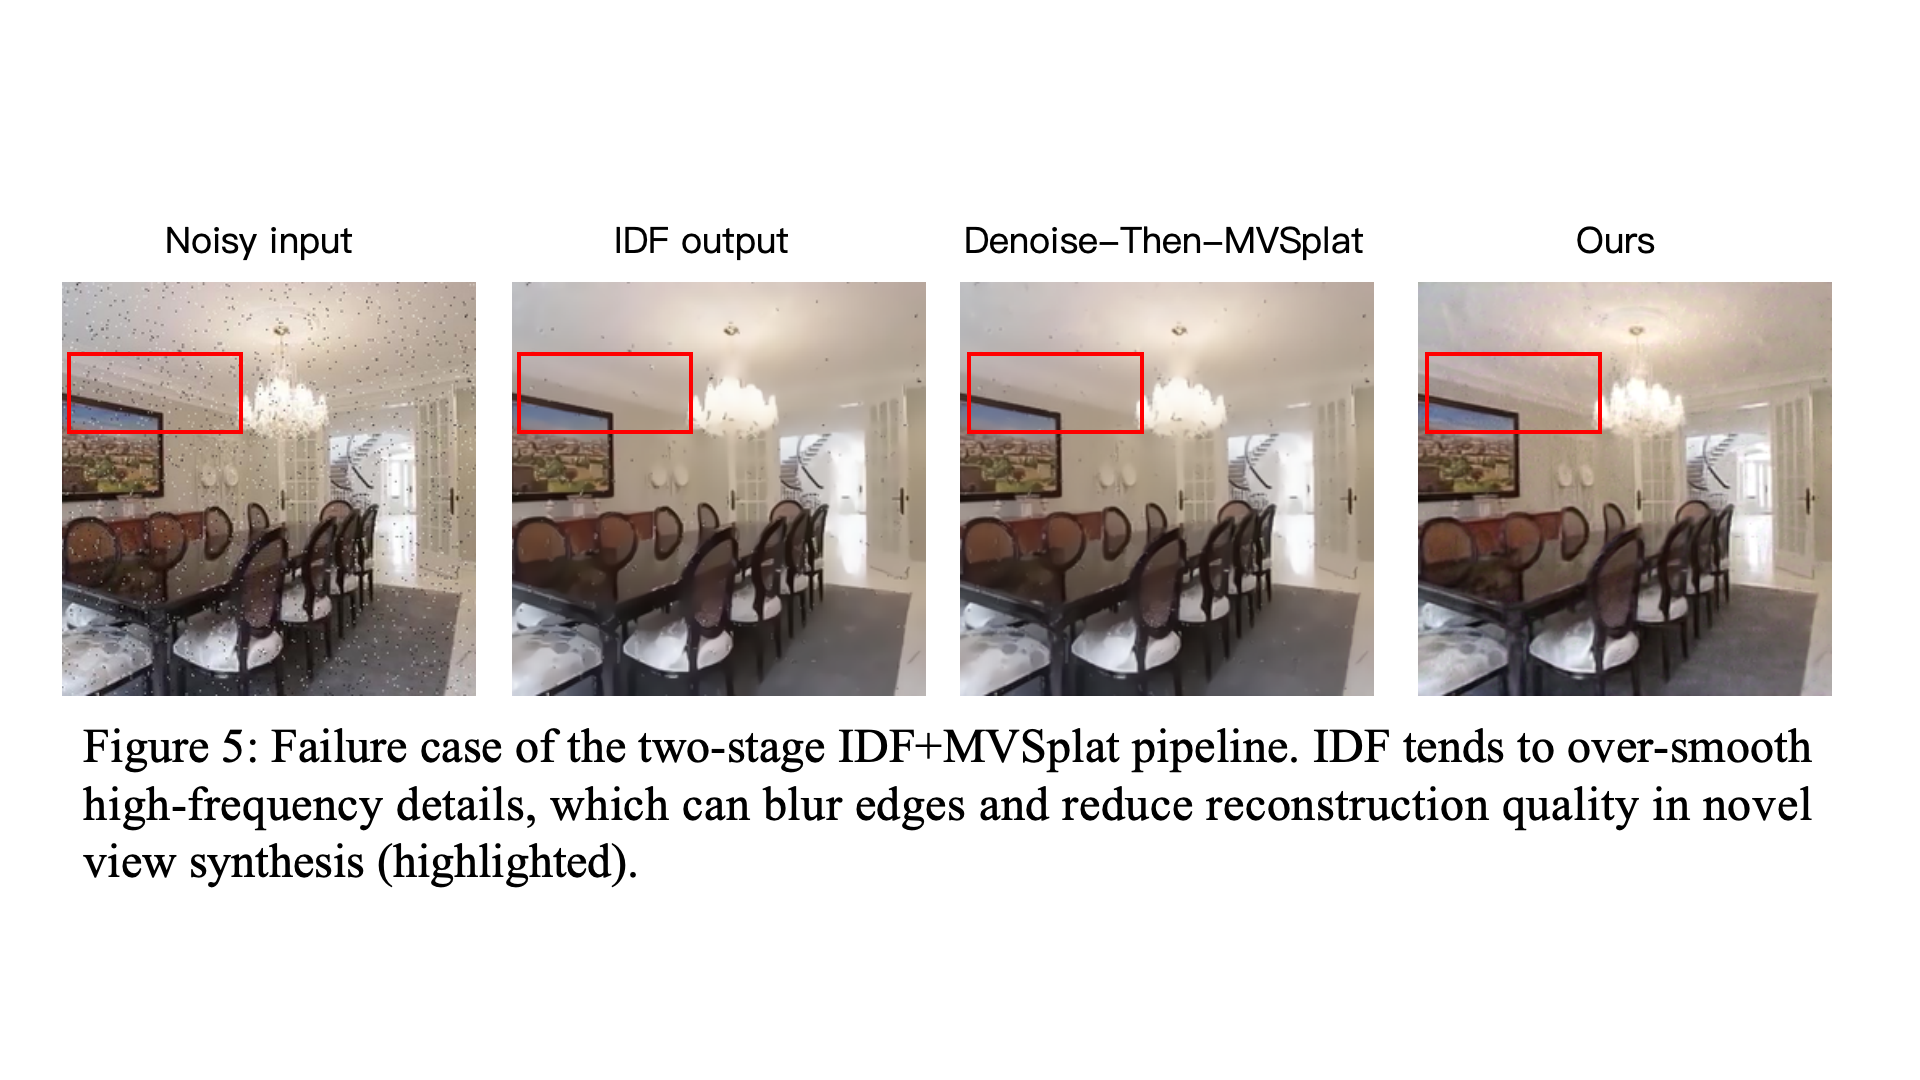
\includegraphics[width=\linewidth, trim=0 200 0 140, clip]{figs/idf_failure.png}
  \label{fig:idf_failure}
\end{figure}



\subsection{Ablation Study}
\label{subsec:ablation}

We ablate robustness along the \emph{noise dimension}, varying noise \emph{type} and \emph{intensity} to examine trends in both metrics and visual artifacts.

\noindent \textbf{Effect of Gaussian noise level}
\label{subsubsec:ablation_gaussian_level}

We vary the Gaussian noise standard deviation
\(\sigma \in \{0.05,\ 0.08,\\\ 0.12,\ 0.15\}\)
and report results in Tab.~\ref{tab:gaussian_ablation}.
As \(\sigma\) increases, PSNR/SSIM decrease and LPIPS increases for all methods.
However, degradation rates differ: \textbf{MVSplat-Noisy} drops sharply for \(\sigma \ge 0.08\), while \textbf{Denoise-Then-MVSplat} remains competitive at low-to-medium noise but degrades faster at higher noise, consistent with front-end 2D denoising losing fine details required by downstream multi-view reconstruction.
In contrast, \textbf{DenoiseSplat} shows a smoother decline and maintains favorable LPIPS even under strong noise, indicating better generalization across noise intensities.

\noindent \textbf{Effect of noise level for other noise types}
\label{subsubsec:ablation_other_level}

We also vary noise hyperparameters for other types: Poisson ($scale$), speckle (multiplicative variance), and salt-and-pepper (\(\alpha \in \{0.01, 0.03\}\)); see Tab.~\ref{tab:other_noise_ablation}.

\begin{table}
  \centering
  \caption{%
    Ablation on the hyper-parameters of other noise types for our DenoiseSplat. 
    Each entry reports performances on the noisy RE10K test set.
  }
  \label{tab:other_noise_ablation}
  \begin{tabular}{lcccc}
    \toprule
    Noise type & Parameter setting & PSNR & SSIM & LPIPS \\
    \midrule
    \multirow{2}{*}{Poisson} & scale $ = 0.03$ & 24.10 & 0.740 & 0.331\\
                             & scale $ = 0.04$ & 23.74 & 0.723 & 0.350\\
    \midrule
    \multirow{2}{*}{Speckle} & $\sigma = 0.02$ & 25.43 & 0.846 & 0.177\\
                             & $\sigma = 0.05$ & 25.36 & 0.832 & 0.211\\
    \midrule
    \multirow{2}{*}{Salt--Pepper} & $\alpha = 0.01$ & 24.98 & 0.816 & 0.241\\
                                  & $\alpha = 0.03$ & 24.53 & 0.776 & 0.298\\
    \bottomrule
  \end{tabular}
\end{table}

\begin{figure*}[t]
  \centering
  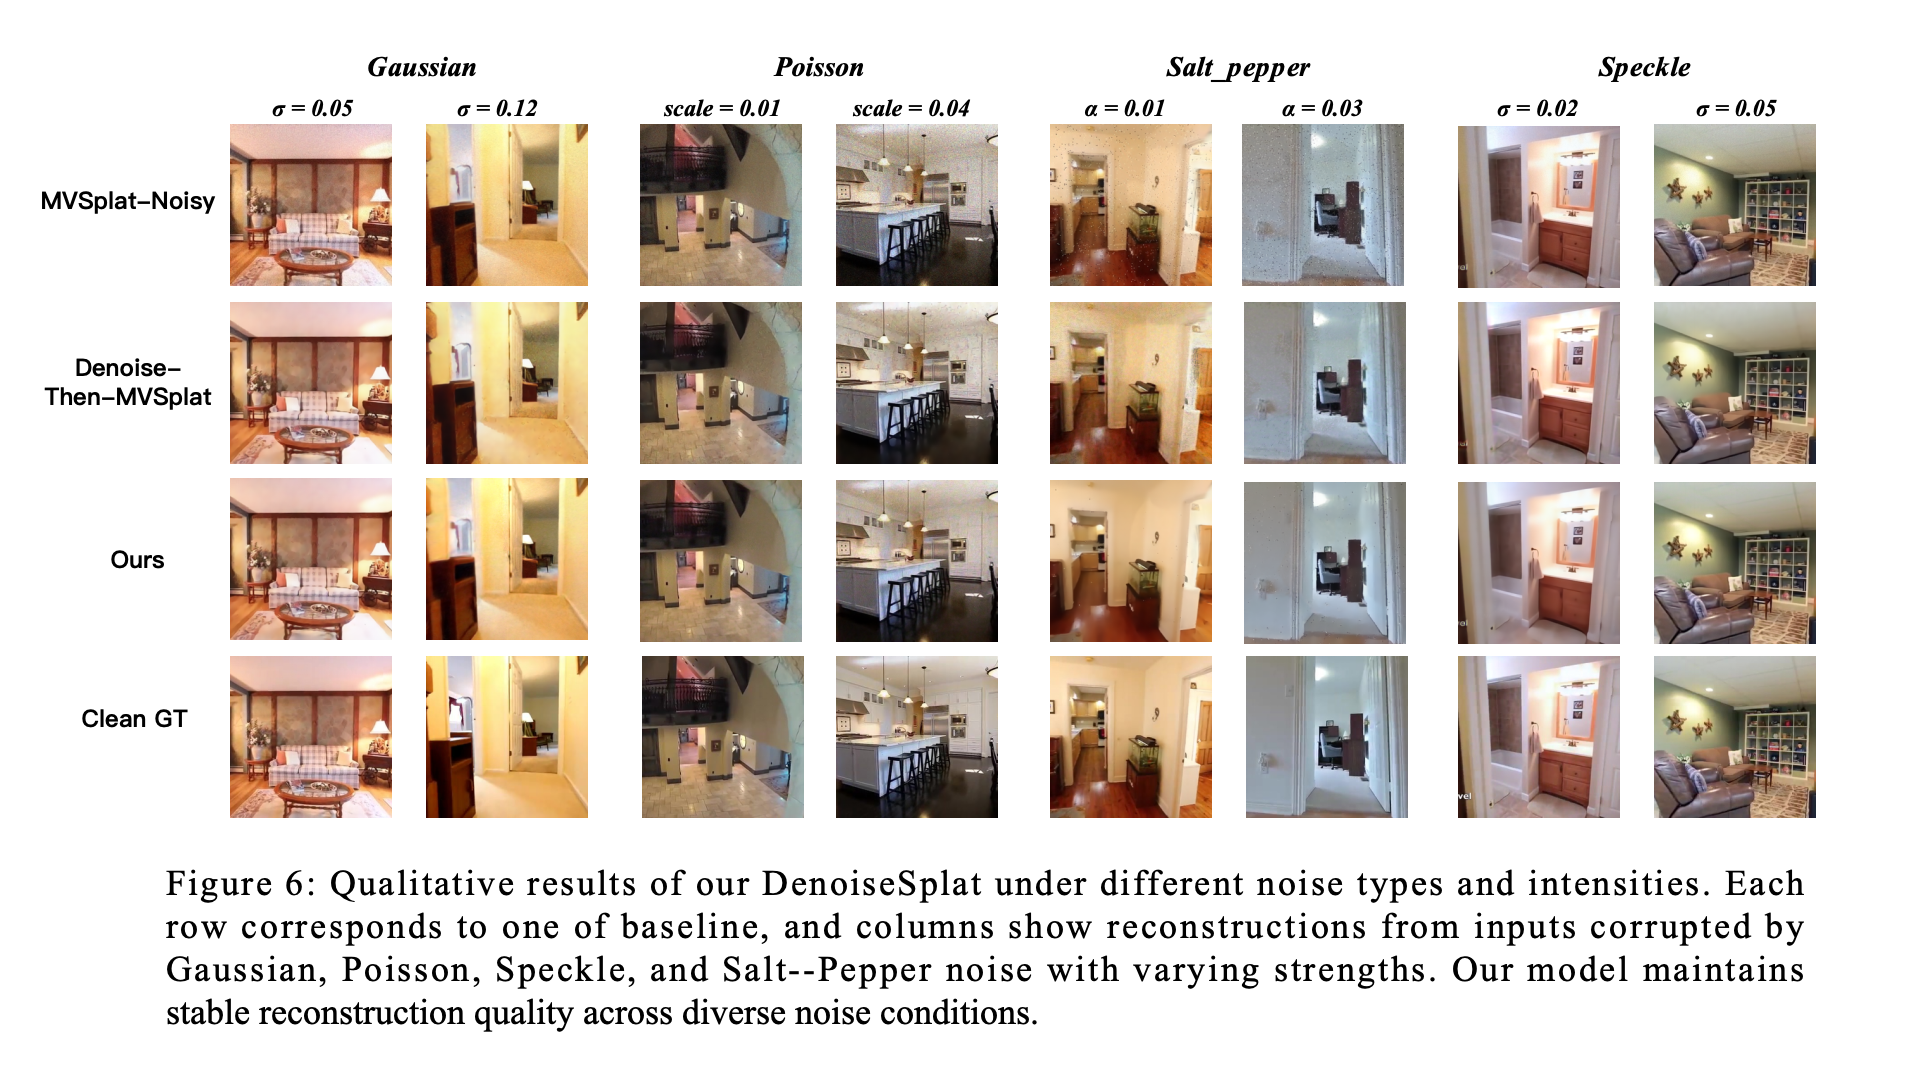
\includegraphics[width=1\linewidth, trim=0 50 0 50, clip]{figs/qualitative_noise.png}
  \label{fig:qualitative_noise}
\end{figure*}


We further include qualitative comparisons in Fig.~6 under representative settings (e.g., Gaussian \(\sigma=0.05\) vs.\ 0.12; Poisson $scale=0.03$ vs.\ 0.04; salt-and-pepper \(\alpha=0.01\) vs.\ 0.03; and speckle low vs.\ high variance).
At low noise, all methods recover main structures but \textbf{MVSplat-Noisy} often leaves residual noise; as noise increases, \textbf{MVSplat-Noisy} exhibits stronger artifacts and instability, \textbf{Denoise-Then-MVSplat} becomes smoother with weakened textures/boundaries, and \textbf{DenoiseSplat} better preserves contours and texture cues with more stable novel-view renderings.

